A mass spectrometer separates the carbon isotopes $^{12}\mathrm{C}^+$ and $^{14}\mathrm{C}^+$. The singly charged ions enter a magnetic field of \BO\ at a speed of \vO, move on a half circle and hit a detector plate (see figure).

\begin{center}
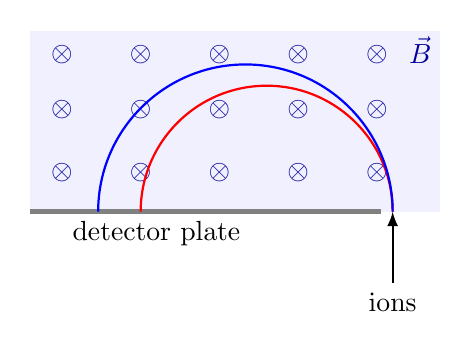
\begin{tikzpicture}[>=latex]
 \fill[blue!6] (-4.6,0) rectangle (0.6,2.3);
 \foreach \x in {-4.2,-3.2,...,0.0} \foreach \y in {0.5,1.3,2.0} \node[blue!60!black] at (\x,\y) {$\otimes$};
 \node[blue!60!black] at (0.35,2.05) {$\vec B$};
 \draw[line width=2pt, gray] (-4.6,0) -- (-0.15,0);
 \node[below] at (-3,0) {detector plate};
 \draw[->, thick] (0,-0.9) node[below] {ions} -- (0,0);
 \draw[red, thick] (0,0) arc (0:180:1.6);
 \draw[blue, thick] (0,0) arc (0:180:1.87);
\end{tikzpicture}
\end{center}

\begin{abcliste}
\abc Calculate the radius of the path of the $^{12}\mathrm{C}^+$ ions.

\abc How far apart do the two isotopes hit the plate?

\abc Which of the two isotopes hits the plate farther from the entrance?
\end{abcliste}
